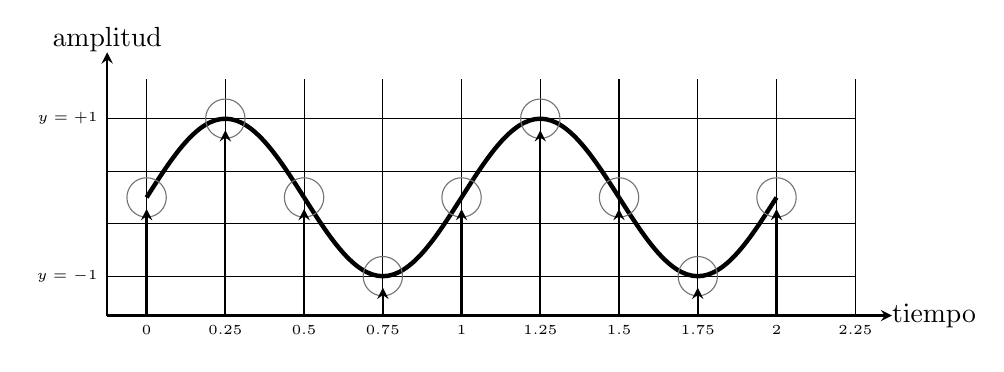
\begin{tikzpicture}
\tikzstyle{stealth} = [-stealth, thick]
\tikzstyle{invisible} = [outer sep=0,inner sep=0,minimum size=0]
\tikzstyle{circle} = [shape=circle, minimum size=0.5cm, draw=black!55]
    \draw (-0.5,1)node[left,font=\tiny] {$y=+1$} -- (9,1);
    \draw (-0.5,-1)node[left,font=\tiny] {$y=-1$} -- (9,-1);
    \draw (-0.5,-0.33)node[left,font=\tiny] {} -- (9,-0.33); 
    \draw (-0.5,0.33)node[left,font=\tiny] {} -- (9,0.33); 
    \foreach \x in {0,0.25,...,2.25}
    {
    	\draw (\x*4,-1.5)node [below,font=\tiny,] {\x } -- (\x*4,1.5) ;
    }
    \draw[ultra thick, ] (0,0) node (v5) {} sin (1,1) node (v7) {};
    \draw[ultra thick, ] (1,1) cos (2,0) node (v9) {};
    \draw[ultra thick, ] (2,0) sin (3,-1) node (v11) {};
    \draw[ultra thick, ] (3,-1) cos (4,0) node (v13) {};
    \draw[ultra thick, ] (4,0)  sin (5,1) node (v15) {};
    \draw[ultra thick, ] (5,1) cos (6,0) node (v17) {};
    \draw[ultra thick, ] (6,0) sin (7,-1) node (v19) {};
    \draw[ultra thick, ] (7,-1) cos (8,0) node (v21) {}; 
\node [invisible] (v1) at (-0.5,-1.5) {};
\node [invisible] (v2) at (-0.5,2) {amplitud};
\node [invisible] (v3) at (10,-1.5) {tiempo};
\draw [stealth] (v1) edge (v2);
\draw [stealth] (v1) edge (v3);
\node [circle] at (0,0) {};
\node [circle] at (1,1) {};
\node [circle] at (2,0) {};
\node [circle] at (3,-1) {};
\node [circle] at (4,0) {};
\node [circle] at (5,1) {};
\node [circle] at (6,0) {};
\node [circle] at (7,-1) {};
\node [circle] at (8,0) {};
\node [invisible] (v4) at (0,-1.5) {};
\node [invisible] (v6) at (1,-1.5) {};
\node [invisible] (v8) at (2,-1.5) {};
\node [invisible] (v10) at (3,-1.5) {};
\node [invisible] (v12) at (4,-1.5) {};
\node [invisible] (v14) at (5,-1.5) {};
\node [invisible] (v16) at (6,-1.5) {};
\node [invisible] (v18) at (7,-1.5) {};
\node [invisible] (v20) at (8,-1.5) {};
\draw [stealth] (v4) edge (v5);
\draw [stealth] (v6) edge (v7);
\draw [stealth] (v8) edge (v9);
\draw [stealth] (v10) edge (v11);
\draw [stealth] (v12) edge (v13);
\draw [stealth] (v14) edge (v15);
\draw [stealth] (v16) edge (v17);
\draw [stealth] (v18) edge (v19);
\draw [stealth] (v20) edge (v21);
\end{tikzpicture}